\label{sec:background}
This section provides a description of how Hipster works and how its subsystem QuickSpec generates conjectures.

\subsection{Theory Exploration in Hipster}
Figure \ref{fig:hipster} gives an overview of the Hipster system. Starting from an Isabelle theory file, defining a set of datatypes and functions, the user calls Hipster on a list of functions about which she is interested in finding lemmas. The workings of Hipster can be divided up into three stages:
\begin{enumerate}
\item Generation of Haskell code. 
\item Theory exploration in Haskell.
\item Proof in Isabelle.
\end{enumerate}
\begin{figure}[htbp]
\begin{center}
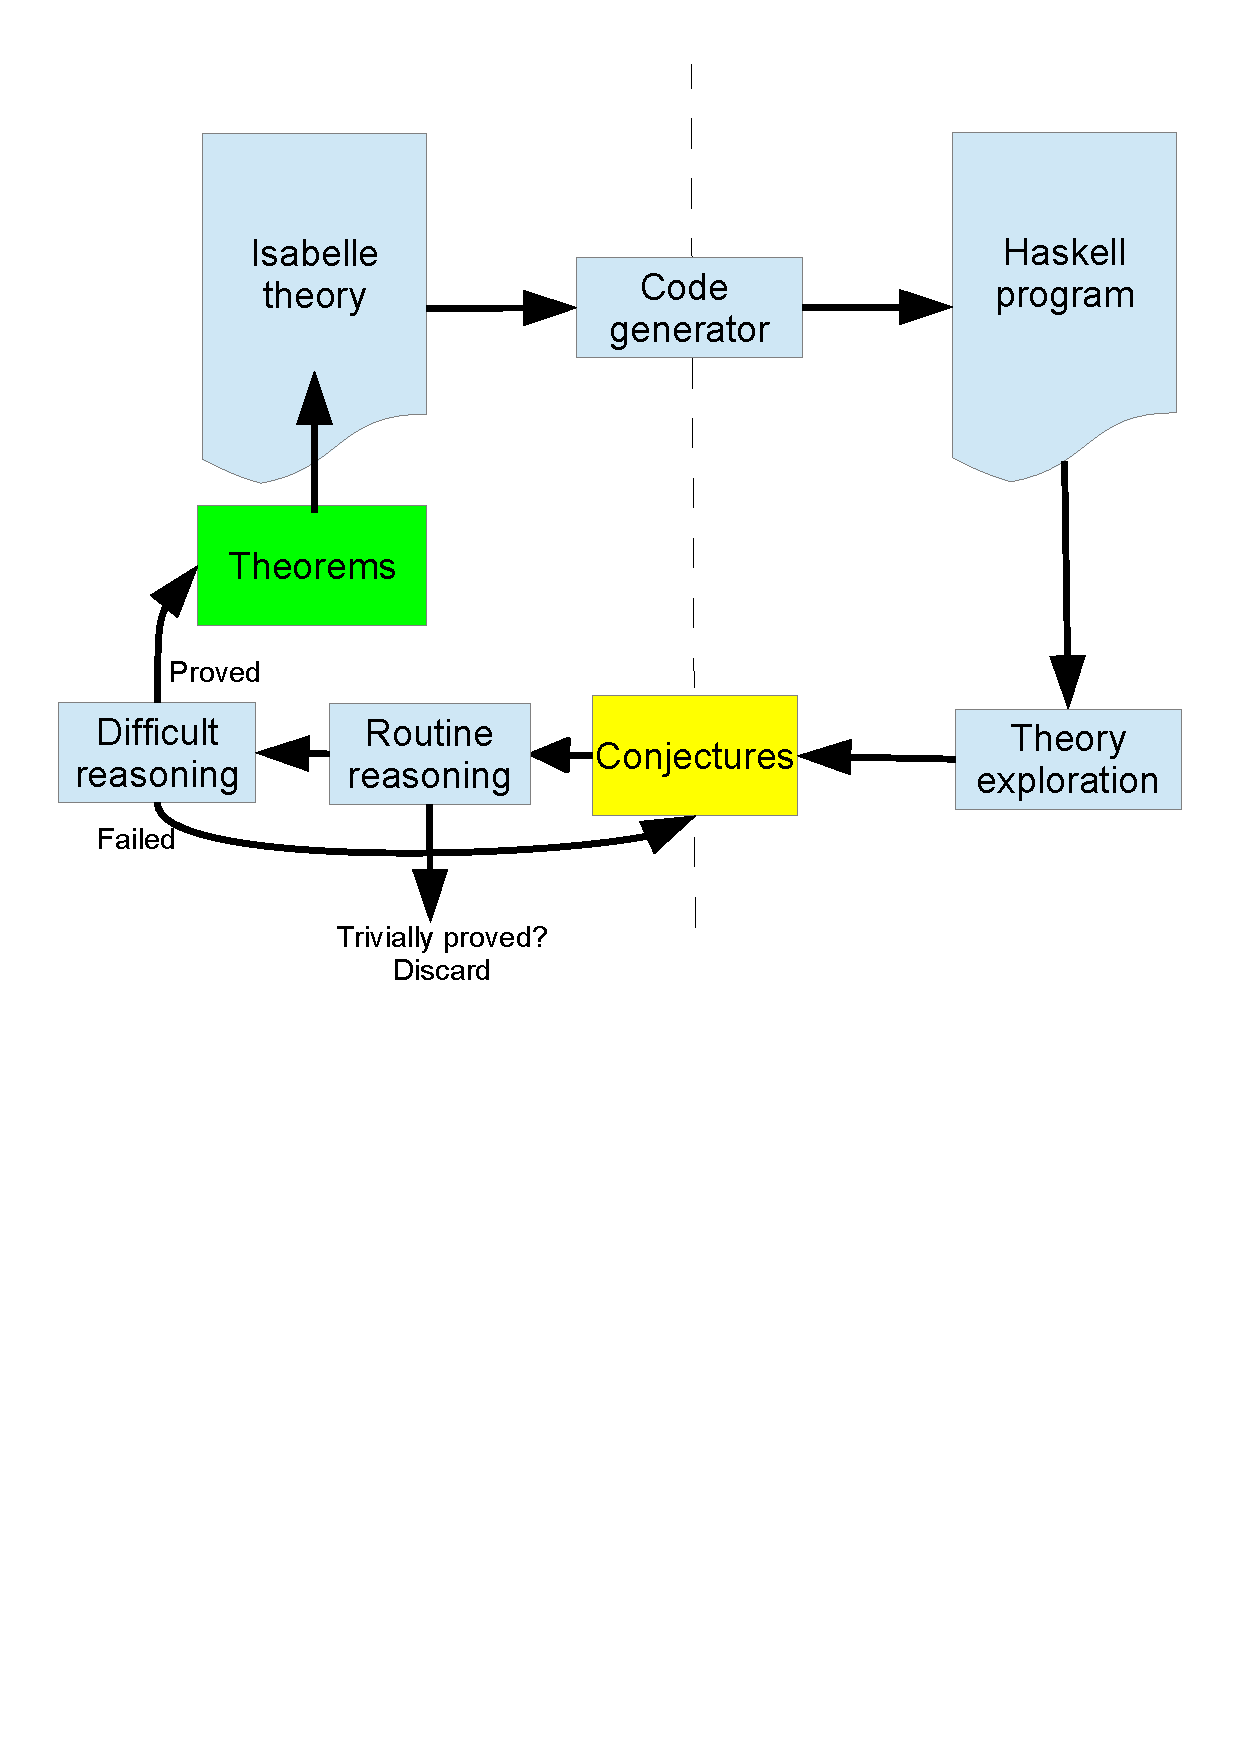
\includegraphics[scale=0.4]{hipster}
\caption{Overview of Hipster}
\label{fig:hipster}
\end{center}
\end{figure}
Hipster uses Isabelle's code generator \cite{codegen2}, to translate the theory to a Haskell program. Hipster then employs the theory exploration system HipSpec as a backend for generating conjectures. While HipSpec can be used also as a fully fledged theorem prover, Hipster only uses its conjecture generation subsystem QuickSpec \cite{quickspec}, and performs proofs inside Isabelle. Isabelle is an LCF-style prover, which means that it is based on a small core of trusted axioms, upon which subsequent proofs must be built. Therefore, any proofs found outside Isabelle, e.g. by HipSpec, would have to be reconstructed inside Isabelle anyway. Hence it is easier for Hipster to simply use Isabelle for proofs in the first place. 

Not all conjectures returned from QuickSpec are interesting. Hipster is parametrised by two tactics, which can be set by the user: one for \emph{routine reasoning} and one for \emph{difficult reasoning}. Conjectures solved by routine reasoning are deemed trivial and discarded, while those requiring more difficult reasoning are displayed to the user and included in the Isabelle theory so they can be used in subsequent proofs if necessary. In the context of this paper, routine reasoning is first-order equational reasoning and simplification, while difficult reasoning involves some kind of induction. Occasionally, Hipster might discover some conjecture which it cannot prove automatically. Such an open conjecture would also be displayed to the user, who can then choose to perform an interactive proof.

\subsection{Conjecture Generation in QuickSpec}
% XXX: "by default three per type" ?
QuickSpec takes as input a set of functions and variables (by default three per type), and generates all type-correct terms up to a given limit (by default depth three). The number of variables and term-depth limit can be adjusted by the user. QuickSpec then proceeds to divide the generated terms into equivalence classes, so that each equivalence class eventually represents a set of equations. Initially, all terms of the same type are in the same equivalence class. QuickSpec then uses QuickCheck \cite{quickcheck}, to generate random ground values for the variables in the terms, and evaluates the result. If two terms in an equivalence class turn out to evaluate differently, the equivalence class is split accordingly. The process is then repeated until the equivalence classes stabilise (after several hundred different random tests), which means that we usually have quite a high confidence in that the conjectures produced are probably true, even though they are not yet proved.  

% This paragraph could possibly be in the next section on conditional lemmas, but it feels like it belongs to the Background section in a way...
The support in QuickSpec for generating conditional conjectures (implications) is still rather basic. In this case, QuickSpec will in addition to the other input require the user to specify a predicate to use as the premise of an implication. Term generation proceeds as described above, but testing takes the given predicate into account. Here, we are only interested in tests with values that make the premise true, otherwise we may split the equivalence classes when they should not be split. QuickCheck uses special functions called \emph{generators} to produce random values of a given type. If using QuickSpec directly in Haskell, the user can program special purpose generators that could be made to only produce values satisfying a given predicate. In Hipster, however, these generator functions are simpler as they have to be automatically derived together with the Haskell code. Tests not satisfying the premise are simply discarded during conditional exploration, which means that we typically must generate more tests than for equational conjectures. Also, the risk of some non-theorem slipping through is slightly higher, but as Hipster then attempts to prove all conjectures, such a statement would be caught in the proving phase. Automatically generating customised generator functions is further work. 

%%% Example if there is space %%%
\subsubsection*{Example}
As a small example, consider a theory exploration attempt where we have asked Hipster for lemmas about a function \texttt{sort}. We are furthermore interested in the case with the condition that the predicate \texttt{sorted} holds (for one variable). %Among the terms generated by QuickSpec are for example: \texttt{xs}, \texttt{sort xs}, \texttt{sort(sort xs)}. 
QuickSpec first performs one pass looking for plain equations, then a second where it considers the condition \texttt{sorted xs}. 

We start with the first phase, where QuickSpec investigates non-conditional conjectures. Among the terms generated by QuickSpec are those in the table below. Initially, all terms are placed in the same equivalence class. Suppose QuickSpec generates the random value \texttt{xs} $\rightarrow$ \texttt{[3,1]}.     

\begin{tabularx}{\textwidth}{l  X  X  X}
 & Term & Ground Instance & Value \\
 \hline
1 \quad &\texttt{sort xs} & \texttt{sort [3,1]} & \texttt{[1,3]} \\
2 \quad&\texttt{sort(sort xs)} &\texttt{sort(sort [1,3])} & \texttt{[1,3]}\\  %% TODO: check this: shouldn't it be sort(sort [3,1])?
3 \quad &\texttt{xs} &\texttt{[3,1]} & \texttt{[3,1]} \\
\end{tabularx}

\noindent Terms 1 and 2 evaluate to the same value and remain in the same equivalence class, while term 3 gets put in a different one. After this, no subsequent tests further split these equivalence classes, and we can read off the equation: \texttt{sort(sort xs) = xs}.  %% TODO: Isn't it sort(sort xs) = sort xs??

In the second phase, QuickSpec performs a new exploration, this time requiring the predicate \texttt{sorted xs} to hold for all test values. Suppose we test with the sorted list: \texttt{xs}$ \rightarrow$ \texttt{[1,2]} (other non-sorted values for \texttt{xs} would be discarded).       

\begin{tabularx}{\textwidth}{l  X  X  X}
 & Term & Ground Instance & Value \\
 \hline
1 \quad &\texttt{sort xs} & \texttt{sort([1,2])} & \texttt{[1,2]} \\
2 \quad&\texttt{sort(sort xs)} &\texttt{sort(sort [1,2])} & \texttt{[1,2]}\\
3 \quad &\texttt{xs} &\texttt{[1,2]} & \texttt{[1,2]} \\
\end{tabularx}

\noindent This time, all terms evaluate to the same value on all tests where the list is sorted, so all three terms remain in the same equivalence class. QuickSpec realises that there is no point producing the conjecture \texttt{sorted xs ==> sort(sort xs) = xs}, as this is subsumed by the non-conditional equation discovered in the first phase. It will however produce the additional conjecture \texttt{sorted xs ==> sort xs = xs}, which clearly only holds if the list is already sorted.

%% TODO: revise example
